
%--------------------------------------------------------------
% ĐẠI HỌC BÁCH KHOA HÀ NỘI
% Trường Điện - Điện tử
% Khoa Tự động hoá
%
% MẪU SOẠN THẢO ĐỒ ÁN

% Phiên bản bổ sung ghi chú sửa đổi, kế hoạch thực hiện và biên bản cuộc họp theo mẫu của thầy Nguyễn Quốc Cường - Smart Sensor Lab
%--------------------------------------------------------------

\documentclass{thesis}
\usepackage[utf8]{inputenc} % 
\usepackage[T5]{fontenc} % Font Vietnamese
\usepackage{graphicx} % Figure
\usepackage{float} % Set position figure or table
\usepackage{mathptmx} % select font Times New Roman
\usepackage{geometry} % Set parameters paper
\usepackage{xcolor}
\usepackage[fontsize=13pt]{scrextend} % set font size = 13pt
% \usepackage{indentfirst} % Indent first line
\usepackage[protrusion=false]{microtype}
\usepackage{titling}
\usepackage{multicol}

\usepackage{amsmath} % for math equation

\usepackage{siunitx} % for unit
\usepackage{longtable} % for long table
% \usepackage{subfigure}
\usepackage{subcaption}

\linespread{1.2}

\nocite{*}


%% START DOCUMENT
\begin{document}

% CREATE COVER PAGE
% CREATE COVER PAGE

\begin{center}
    \vspace{12pt} % line spacing
        \textbf{\fontsize{15pt}{0pt} \selectfont{} ĐẠI HỌC BÁCH KHOA HÀ NỘI }
    \vspace{0.5cm}
    
% INSERT LOGO
\begin{figure}[H]
    \centering
    \includegraphics[width=2cm,height=3cm]{logoBK.png}
\end{figure}

% THESIS TYPE
\vspace{48pt}
        \fontsize{25pt}{0pt}{\fontfamily{qag}\selectfont{} \textbf{ĐỒ ÁN TỐT NGHIỆP}
}
\vspace{24pt}

 % THESIS TITTLE
        \fontsize{17pt}{0pt}{\fontfamily{qag}\selectfont{} \textbf{   
        THIẾT KẾ THIẾT BỊ ĐỌC GHI
        MÀN HÌNH CỘT BƠM \\ XĂNG DẦU
        }}
\vspace{18pt}

% NAME
        \fontsize{14pt}{0pt}\selectfont{} \textbf{NGUYỄN THÁI SƠN}
    \vspace{3pt}

% EMAIL    
        \fontsize{14pt}{0pt}\selectfont{} son.nt212951@sis.hust.edu.vn
    \vspace{12pt} % line spacing

% MAJOR
        \fontsize{14pt}{0pt}\selectfont{} \textbf{Ngành Kỹ thuật Điều khiển và Tự động hóa}  
\end{center}
    \vspace{48pt}

% INFORMATION: SUPERVISOR NAME, STUDENT NAME,...
\begin{table}[H]
    \centering
        \begin{tabular}{l l c}
            \textbf{Giảng viên hướng dẫn:}    &  PGS.TS. Nguyễn Quốc Cường \vspace{6pt} & \\
            &\vspace{3pt} & \fontsize{10pt}{0pt}\selectfont{} Chữ ký của GVHD \\
            \textbf{Khoa:} & Tự động hóa \vspace{3pt}\\ 
            \textbf{Trường:} & Điện - Điện tử
        \end{tabular}
\end{table}

% TIME
\begin{center}
    \vspace{48pt}
    \fontsize{14pt}{0pt}\selectfont{} \textbf{Hà Nội, 3/2025}
\end{center}
    \newpage
   %     \clearpage
%            \thispagestyle{empty}
  %              \cleardoublepage

% THESIS TASK                
% THESIS TASK                
\begin{multicols}{2}
\centering
\hspace{-3cm}BỘ GIÁO DỤC \& ĐÀO TẠO \\ \hspace{-3cm}\textbf{ĐH BÁCH KHOA HÀ NỘI}

\columnbreak

\hspace{-1.6cm}\textbf{CỘNG~HÒA~XÃ~HỘI~CHỦ~NGHĨA~VIỆT~NAM} \\ \hspace{-1.6cm}\textbf{Độc lập -- Tự do -- Hạnh phúc}

\end{multicols}

\begin{center}
   \textbf{NHIỆM VỤ \\ĐỒ ÁN TỐT NGHIỆP} 
\end{center}

%\raggedright

\hspace{-1cm}Họ và tên sinh viên: Nguyễn Thái Sơn\\Khóa: K66 \hfill Trường: Điện -- Điện tử \hfill Ngành: KT ĐK \& TĐH
    
    % Thay các dấu chấm (\ldots) dưới đây bằng nội dung
    
    \hspace{-1cm}\textit{1. Tên đề tài}\\
             Thiết kế thiết bị đọc ghi màn hình cột bơm xăng dầu  \\[0.2cm]
    \textit{2. Nội dung đề tài}\\
            Thiết kế và triển khai hệ thống gồm phần cứng và phần mềm
            để thu dữ liệu hiển thị trên màn hình cây xăng, giải mã
            và lưu các lượt bơm xăng. Lấy mẫu thông tin màn hình với tần số 100Hz. Có kết nối mạng LAN với máy tính nội bộ. Thiết bị có giao diện giám sát và điều khiển dạng Web App.

            Các công việc bao gồm:
            \begin{itemize}
                \item Thiết kế mạch thu dữ liệu màn hình
                \item Thu thập và phân tích tín hiệu gửi tới màn hình
                \item Thiết kế bộ giải mã dữ liệu
                \item Triển khai hệ thống mạng và phần mềm để thu và giải mã dữ liệu màn hình theo thời gian thực
                \item Triển khai cơ sở dữ liệu và giao diện hiển thị dữ liệu màn hình
                \item Chạy kiểm thử hệ thống tại hiện trường
            \end{itemize}
           
    \textit{3. Thời gian giao đề tài: 18/02/2025} \\[0.2cm]

    \textit{4. Thời gian hoàn thành: dd/mm/yyyy} \\[0.2cm]

\vspace{6pt}
\hspace{7cm}\textit{Ngày (dd) tháng (mm) năm 202y}\\
\vspace{2pt}
\hspace{8.5cm}\textbf{CÁN BỘ HƯỚNG DẪN} \\

\vspace{36pt}

\hspace{8cm}\textbf{Nguyễn Quốc Cường}
    \newpage
%        \clearpage
 %           \thispagestyle{empty}
 %               \cleardoublepage    
                
% THANKS
% THANKS
\section*{LỜI CẢM ƠN}
    \thispagestyle{empty}
Đây là mục tùy chọn, nên viết phần cảm ơn ngắn gọn, tránh dùng các từ sáo rỗng.

\vspace{6pt}
    \hspace{7cm}Hà Nội, ngày 24 tháng 03 năm 2025
        
        \hspace{8.6cm} Sinh viên thực hiện      % command '\hspace' used to line indents

\vspace{2cm}
    \hspace{8.8cm}\textbf{Nguyễn Thái Sơn} % change name

\newpage % create a new page
%    \thispagestyle{empty} 
%        \clearpage
%            \thispagestyle{empty}
  %              \cleardoublepage

% SUMMARY PART
% SUMMARY PART
\section*{TÓM TẮT ĐỒ ÁN}
    \thispagestyle{empty}
(Sẽ được bổ sung vào giai đoạn cuối của đồ án)


\newpage

% TABLE OF CONTENT
\tableofcontents 
    \thispagestyle{empty}
        \newpage
 %           \thispagestyle{empty}
  %              \cleardoublepage

% LIST OF SYMBOLS AND ABBREVIATIONS
\pagenumbering{roman}   % Roman numbering: i, ii, iii, iv,...
\section*{DANH MỤC KÝ HIỆU VÀ CHỮ VIẾT TẮT}
    \phantomsection \addcontentsline{toc}{section}{\numberline{} DANH MỤC KÝ HIỆU VÀ CHỮ VIẾT TẮT}

% Create table
\begin{tabular}{ l l }
    \hspace{1cm} HESS & \hspace{4cm} Hybrid Energy Storage System \\  
    \hspace{1cm} SC & \hspace{4cm} Super Capacitor    \\
    \hspace{1cm} EMS  & \hspace{4cm} Energy Management Strategy 
\end{tabular}  
    \newpage

% LIST OF FIGURES
{\let\oldnumberline\numberline
    \renewcommand{\numberline}{Hình~\oldnumberline}
        \listoffigures}
            \phantomsection\addcontentsline{toc}{section}{\numberline{} DANH MỤC HÌNH VẼ}
\newpage

% LIST OF TABLES
{\let\oldnumberline\numberline
    \renewcommand{\numberline}{Bảng~\oldnumberline}
        \listoftables}
            \phantomsection\addcontentsline{toc}{section}{\numberline{} DANH MỤC BẢNG BIỂU}
\newpage

%%%%%%%%%%%% Using for lab report version %%%%%%%%%%%%
\section*{Bảng cập nhật báo cáo} \label{edit_note}

\begin{center}
    \begin{longtable}{|>{\centering\arraybackslash}p{1cm}|>{\raggedright\arraybackslash}p{4cm}| >{\raggedright\arraybackslash}p{10cm}|}
    \caption{Bảng cập nhật báo cáo.}
    \\
        \hline
        \textbf{Ngày} & \textbf{Nội dung báo cáo} & \textbf{Sửa đổi / ghi chú} \\
        \hline
        \endhead
      
        4/3 & Bảng kế hoạch & Lập bảng kế hoạch công việc \\

        24/3 & Chương 1: Tổng quan hệ thống & Viết nội dung tổng quan hệ thống \\

        25/3 & Meeting note & Ghi các meeting note vào báo cáo \\

        \hline
    \end{longtable}
\end{center}
\thispagestyle{empty}
\newpage

\section*{Kế hoạch thực hiện} \label{Implementation_plan}

\begin{longtable}{|>{\centering\arraybackslash}p{1cm}| >{\raggedright\arraybackslash}p{3cm}| >{\raggedright\arraybackslash}p{7cm}| > {\raggedright\arraybackslash}p{3cm}|}
    \caption{Bảng kế hoạch dự án.}
    \label{tab:plan_project}
    \\
        \hline
        Tuần & Nhiệm vụ & Yêu cầu cần đạt & Trạng thái \\
        \endhead
        
        \hline
        26 & Xác định mục tiêu đề tài & Liệt kê yêu cầu bài toán, chức năng thiết bị & Hoàn thành \\
        
        \hline
        27 & Tìm hiểu đặc điểm cột bơm, xác định phạm vi bài toán & Báo cáo trình bày đặc điểm cột bơm & Hoàn thành \\

        \hline
        28 & Lập bảng kế hoạch công việc & File Excel có bảng liệt kê các đầu việc chi tiết cho các tuần cùng với tiến độ được cập nhật &  Hoàn thành \\
        
        \hline
        29 & Vẽ sơ đồ hệ thống & Sơ đồ tổng quan hệ thống & Hoàn thành \\

        \hline
        30 & Liệt kê và tìm hiểu các công nghệ sử dụng & Báo cáo tìm hiểu các phần tử IC được sử dụng, CPLD và STM32 & Hoàn thành \\

        \hline 
        31 & Tìm hiểu mạch cứng & Đọc hiểu và viết tài liệu về mạch cứng, tìm hiểu các linh kiện & Đang thực hiện \\

        \hline
        32 & Vẽ thiết kế mạch cứng & Bản thiết kế mạch cứng & Chưa làm \\
        
        \hline 
        32 & Triển khai hệ thống phần mềm & Xây dựng kiến trúc source code và chuẩn API & Chưa làm \\

        \hline
        33 & Triển khai  backend server & Demo backend server giao tiếp bằng chuẩn API đã đưa ra & Chưa làm \\

        \hline 
        34 & Triển khai giao diện hiển thị & Demo giao diện mô phỏng màn hình cây xăng theo thời gian thực & Chưa làm\\

        \hline 
        35 & Kiểm thử, chạy thử hệ thống và quay video demo & Demo chạy thử toàn hệ thống, trình bày các lỗi phát sinh nếu có & Chưa làm \\
        
        \hline 
        36 & Viết báo cáo quyển & Trình bày quyển & Chưa làm \\

        \hline 
        37 & Viết báo cáo dạng báo cáo khoa học & Trình bày báo cáo & Chưa làm \\

        \hline

\end{longtable}
\thispagestyle{empty}
\newpage

\section*{Biên bản cuộc họp} \label{tab:Meeting_notes}

\begin{longtable}{|>{\centering\arraybackslash}p{1cm}| >{\raggedright\arraybackslash}p{4cm}| >{\raggedright\arraybackslash}p{5cm}| > {\raggedright\arraybackslash}p{4cm}|}
    \caption{Biên bản cuộc họp.}
        \\
        \hline
        Ngày & Nội dung & Quyết định & Nhiệm vụ tiếp theo \\
        \endhead
       
        \hline
        25/2 & Giao đề tài và nêu ý tưởng chung về đề tài & Đưa ra các đầu việc, thống nhất về đầu mối & Tìm hiểu công nghệ, dựng hệ thống và tài liệu hóa  \\

        \hline
        4/3 & Trình bày sơ bộ về tiến độ, bảng kế hoạch (đã đưa và đang chờ duyệt). Thống nhất lịch họp hàng tuần & Khoảng hết tuần 5, đầu tuần 6 báo cáo overview và kế hoạch đồ án & Bắt đầu viết tài liệu hệ thống \\

        \hline
\end{longtable}
\thispagestyle{empty}
\newpage

%%%%%%%%%%%%%%%%%%%%%%%%%%%%%%%%%%%%%%%%%%%%%%%%%%%%%%%%%%%%

%% --------------------------------------------------%%
%------------CHAPTER 1---------------------------%
%%-----------------------------------------------------%

\pagenumbering{arabic} % numbering: 1,2,3,...
    \section*{CHƯƠNG 1. GIỚI THIỆU CHUNG} 
        \addcontentsline{toc}{section}{\numberline{}CHƯƠNG 1. GIỚI THIỆU CHUNG} % Reference to content

\setcounter{section}{1} 
    \setcounter{subsection}{0}
        \setcounter{figure}{0}
            \setcounter{table}{0}
%%--------------------------------------------------------

\subsection{Vai trò của thiết bị đọc ghi màn hình cột bơm xăng dầu}

\hspace{1cm} Công nghệ số mang đến ngày càng nhiều lợi ích to lớn về mặt tiện dụng, hiệu quả và tiết kiệm thời gian cho doanh nghiệp cũng như người dùng. Từ đó, nhu cầu lớn về chuyển đổi số được phát sinh. Các thông tin giao dịch, hóa đơn trên giấy tờ ngày càng được thay thế bằng các giao dịch, hóa đơn điện tử, thuận tiện cho truyền tải thông tin, lưu trữ và quản lý. Các hệ thống trạm xăng và cột bơm cũng không phải ngoại lệ với nhu cầu đó, các giao dịch, lượt bơm xăng cũng cần được ghi lại dưới dạng dữ liệu số để gửi lên máy chủ của doanh nghiệp, thuận tiện lưu trữ và thống kê một cách chính xác, ổn định và giảm hoặc triệt tiêu những lỗi con người có thể gây ra.

Những cột bơm mới được bán gần đây cũng đã được sản xuất tích hợp chức năng xuất hóa đơn điện tử. Nhưng còn một lượng rất lớn những cây xăng với công nghệ cũ vẫn còn đạt tiêu chuẩn và sử dụng tốt được ở nhiều trạm bơm trên khắp cả nước, việc bỏ hẳn những cây xăng này đi thay bằng những cây xăng công nghệ mới sẽ tốn nhiều thời gian và chi phí đầu tư, gây lãng phí cũng như thải nhiều rác thải điện tử hơn cho môi trường. Từ đó xuất hiện nhu cầu cải tiến những cây xăng cũ để xuất được hóa đơn điện tử, chi phí và thời gian doanh nghiệp bỏ ra sẽ được tối ưu hơn.

Từ yêu cầu trực tiếp của doanh nghiệp, báo cáo này được viết để đưa ra phương án thiết kế và triển khai hệ thống có thể đọc ghi và phân tích dữ liệu màn hình cây xăng, từ đó phát hiện được các lần giao dịch và lưu trữ, quản lý các lượt giao dịch - lượt bơm xăng đó.


\subsection{Khái quát về yêu cầu và chức năng của hệ thống}

 \hspace{1cm} 

 \textbf{1. \quad Giám sát số liệu hiển thị trên cột bơm theo thời gian thực}

 Hệ thống có thể đọc và hiển thị trực tiếp dữ liệu cột bơm theo thời gian thực bao gồm: số tiền, số lít và đơn giá. Người dùng có thể theo dõi trạng thái hiển thị của cột bơm ngay tại phòng điều khiển mà không cần quan sát trực tiếp màn hình cột.
 

 \textbf{
    2. \quad  Phát hiện các lượt bơm hoàn chỉnh
 }

 Thông qua các số liệu thời gian thực (số tiền, số lít, đơn giá) của cột bơm, hệ thống phát hiện được đâu là bắt đầu và kết thúc của một lượt bơm xăng, thông báo một lượt bơm/hóa đơn hoàn chỉnh.


 \textbf{
    3. \quad Lưu trữ và hiển thị các lượt bơm
 }

 Các lượt bơm được lưu trữ trong cơ sở dữ liệu, tạo cơ sở để có thể xuất các hóa đơn điện tử.


 \textbf{
    4. \quad Hỗ trợ điều khiển từ xa
 }

 Việc ghi dữ liệu cột bơm có thể được điều khiển bật tắt từ xa, thông qua giao diện phần mềm.


 \textbf{
    5. \quad Cập nhật phần mềm từ xa (OTA)
 }

 Hỗ trợ cập nhật phần mềm từ xa, cho phép người dùng cập nhật phiên bản mới từ giao diện người dùng để có tối ưu những tính năng, tiện ích mới nhất từ phiên bản phần cứng đã có.

Thông qua việc triển khai mục tiêu trên, đề tài hướng tới tạo ra một hệ thống đọc và giải mã màn hình cây xăng hoàn chỉnh, đáp ứng nhu cầu quan sát từ xa các cột bơm theo thời gian thực, tự động phát hiện và ghi lại được các lượt bơm, tạo tiền đề để phát triển các ứng dụng như là xuất hóa đơn điện tử, thanh toán không chạm, và các ứng dụng khác.

\subsection{Phạm vi nghiên cứu}

\hspace{1cm} Thiết bị đọc ghi màn hình cột bơm xăng dầu có thể đọc ghi và giải mã loại cột bơm truyền thống có đặc điểm sau:
\begin{itemize}
   \item Hãng sản xuất: ZCheng
   \item Loại cáp màn hình: 8P 3.96mm
   \item Số lượng chân cáp: 8
   \item Số chân tín hiệu của cáp: 3
   \item Giao thức: SPI
   \item Độ lớn frame: 22 byte
   \item Bit rate: 400Kb/s
   \item Tần số frame: 100Hz
\end{itemize}
Đây là loại cột bơm cũ phổ biến tại các trạm xăng trên thị trường. Phạm vi chức năng của hệ thống bao gồm:

 \textbf{1. \quad Giám sát số liệu hiển thị trên cột bơm theo thời gian thực}

 Thu và giải mã dữ liệu SPI gửi tới màn hình thiết bị. Hiển thị giá trị màn hình (số tiền, số lít, đơn giá) theo thời gian thực trên giao diện người dùng.

  \textbf{
    2. \quad  Phát hiện các phiên bơm hoàn chỉnh
 }

 Sau khi bơm xăng, người vận hành dừng bơm một thời gian (5s) hoặc nhấn nút reset để bắt đầu phiên bơm mới, thiết bị phát hiện và ghi lại giá trị màn hình hiện tại thành một phiên bơm.

  \textbf{
    3. \quad Lưu trữ và hiển thị các lượt bơm
 }

 Các bản ghi phiên bơm được lưu vào cơ sở dữ liệu ngay trên máy tính nội bộ và hiển thị lên giao diện quản lý

 \textbf{
    4. \quad Hỗ trợ điều khiển từ xa
 }

Thiết bị đọc màn hình cây xăng có 2 relay đóng ngắt có thể nối nối tiếp vào cột bơm. Từ giao diện quản lý, có thể điều khiển relay đóng ngắt bằng nút ấn trên giao diện.


 \textbf{
    5. \quad Cập nhật phần mềm từ xa (OTA)
 }

 Từ giao diện quản lí, có thể tải (upload) file phần mềm dạng mã nhị phân, gửi cho thiết bị đọc màn hình để thiết bị tự cập nhật. 

\subsection{Giải pháp đề xuất}




\newpage
%---------------------------------------------------------%%
%% ----------CHAPTER 2 -------------------%%
%---------------------------------------------------------%%

\section*{CHƯƠNG 2. CƠ SỞ LÝ THUYẾT}
    \addcontentsline{toc}{section}{\numberline{} CHƯƠNG 2. CƠ SỞ LÝ THUYẾT}

\setcounter{section}{2}
    \setcounter{subsection}{0}
        \setcounter{figure}{0}
            \setcounter{table}{0}
%---------------------------------------------------------%


\newpage

%% --------------------------------------------------%%
%------------CHAPTER 3---------------------------%
%%-----------------------------------------------------%

\section*{CHƯƠNG 3. PHƯƠNG PHÁP LUẬN}
    \addcontentsline{toc}{section}{\numberline{}CHƯƠNG 3. PHƯƠNG PHÁP LUẬN}
    
\setcounter{section}{3}
    \setcounter{subsection}{0}
        \setcounter{figure}{0}
            \setcounter{table}{0}
%%-------------------------------------------------------%%
% --------------------------------------------------------%
%---------------------------------------------------------%


\newpage
%% --------------------------------------------------%%
%------------ CHAPTER 4 ---------------------------%
%%-----------------------------------------------------%

\section*{CHƯƠNG 4. TRIỂN KHAI VÀ THỬ NGHIỆM}
    \addcontentsline{toc}{section}{\numberline{} CHƯƠNG 4. MÔ PHỎNG VÀ KẾT QUẢ}
\setcounter{section}{4}
    \setcounter{subsection}{0}
        \setcounter{figure}{0}
            \setcounter{table}{0}
                \setcounter{equation}{0}

%--------------------------------------------------------%

\subsection{Quy trình triển khai}

\hspace{0.8cm} Ở chương này em trình bày chi tiết quá trình triển khai, xây dựng sản phẩm sử dụng các công nghệ đã lựa chọn ở Chương 2 và dựa trên thiết kế chi tiết đã nêu ra ở Chương 3.

Nội dung gồm quy trình triển khai, mô tả đầu ra sản phẩm,
kiểm thử và chạy với dữ liệu mô phỏng, lắp ráp và kiểm thử tại hiện trường.

\subsubsection{Mạch phần cứng thiết bị đọc màn hình}

\textbf{a. Vẽ mạch PCB từ sơ đồ nguyên lý}

Từ sơ đồ nguyên lý đã đã nêu ở Chương 3, tiến hành vẽ mạch PCB trên Altium:

\begin{figure}[!ht]
    \centering
    \includegraphics[width=0.8\linewidth]{Figures/PCB_top-down.png}
   
    \caption{Mạch PCB - Mặt trên}
    \label{fig:PCB_top-down}
\end{figure}

\begin{figure}[!ht]
    \centering
    \includegraphics[width=0.4\linewidth]{Figures/PCB_side-view.png}
    \hspace{0.1\textwidth}
    \includegraphics[width=0.4\textwidth]{Figures/PCB_bottom-up.png}
    \caption{Mạch PCB - Mặt ngang và mặt dưới}
    \label{fig:PCB_side-view-and-bottom-up}
\end{figure}

\FloatBarrier
\textbf{ b. In và hàn mạch thực tế}
\begin{figure}[!ht]
    \centering
    \includegraphics[width=0.8\linewidth]{Figures/Device_product-top-down.jpg}
    \caption{Sản phẩm thiết bị đọc ghi màn hình cột bơm: mặt trên}
    \label{fig:Device_product-top-down}
\end{figure}

\begin{figure}[!ht]
    \centering
    \includegraphics[width=0.45\linewidth]{Figures/Device_product-bottom-view.jpg}
    \hspace{0.02\textwidth}
    \includegraphics[width=0.45\textwidth]{Figures/Device_product-side-view.jpg}
    \caption{Sản phẩm thiết bị đọc ghi màn hình cột bơm: mặt ngang và dưới}
    \label{fig:device_product}
\end{figure}


\subsubsection{Firmware thiết bị đọc màn hình}

Môi trường/ công cụ phát triển để lập trình cho STM32: STM32CubeIDE.

\textbf{Setup các cổng IO}

\begin{figure}[!ht]
    \centering
    \includegraphics[width=1.0\linewidth]{Figures/Device_stm32-io-config.png}
    \caption{Triển khai: cấu hình các chân trong STM32CubeIDE}
    \label{fig:Device_stm32-io-config}
\end{figure}

Các ngoại vi được sử dụng bao gồm:
\begin{itemize}
    \item SPI1: Kết nối với module W5500, giao tiếp Ethernet.
    \item SPI2: Kết nối với CPLD, nhận dữ liệu màn hình dạng byte data.
    \item USART2: Sử dụng để debug (kết nối với máy tính và gửi thông báo lên màn hình terminal)
    \item Các cổng IO khác:
    \begin{itemize}
        \item PB12 và PB13: điều khiển relay 1 và 2.
        \item PA1, PA2 và PA3: các đèn báo led.
        \item PA9: CPLD Enable
        \item PC9: Frame Stop - Ngắt GPIO đầu vào báo kết thúc 1 frame 
    \end{itemize}
\end{itemize}

\FloatBarrier
\textbf{Triển khai firmware}

 \hspace{0.8cm} Về tổ chức các thư mục, tại thư mục \texttt{core/Src} tổ chức thành 4 thư mục lớn chứa 4 modules được nêu trong phần Kiến trúc triển khai firmware (xem hình minh họa ở chương trước) là: \texttt{capture\_driver}, \texttt{device\_driver}, \texttt{internet} và \texttt{fota}

 Các thuật toán quan trọng bao gồm:

 \begin{itemize}
    \item Khởi tạo và kết nối với phần mềm Device Service
    \item Xử lý ngắt SPI1: Nhận yêu cầu từ Device Service
    \item Xử lý ngắt SPI2: Nhận SPI byte từ CPLD
    \item Xử lý ngắt báo Frame Stop: Báo kết thúc 1 screen frame và tiến hành lưu frame
 \end{itemize}


\begin{figure}[!ht]
    \centering
    \includegraphics[width=1.0\linewidth]{Figures/flowcharts-Device_Receive-screen-frame.png}
    \caption{Thuật toán xử lý ngắt nhận dữ liệu màn hình}
    \label{fig:flowcharts-Device_Receive-screen-frame}
\end{figure}


\begin{figure}[!ht]
    \centering
    \includegraphics[width=1.0\linewidth]{Figures/flowcharts-Device_handle-DS-req.png}
    \caption{Thuật toán xử lý ngắt nhận dữ yêu cầu Device Service}
    \label{fig:flowcharts-Device_handle-DS-req}
\end{figure}
 

\begin{figure}[!ht]
    \centering
    \includegraphics[width=1.0\linewidth]{Figures/flowcharts-Device_Main loop.png}
    \caption{Thuật toán cho chương trình chính}
    \label{fig:flowcharts-Device_Main loop}
\end{figure}

\FloatBarrier

Cấu trúc gói tin giao tiếp giữa Thiết bị đọc ghi màn hình (Device) và Phần mềm giải mã (Device Service) được nêu trong bảng \ref{tab:device-packet_structure}

\begin{table}[h!]
\centering
\begin{tabular}{|c|c|c|p{7cm}|}
\hline
\textbf{Trường} & \textbf{Kích thước} & \textbf{Offset} & \textbf{Mô tả} \\
\hline
Packet Length & 2 bytes & 0–1 & Tổng chiều dài gói tin trừ đi 12 byte đầu (độ dài Payload). \\
\hline
Device MAC & 6 bytes & 2–7 & Địa chỉ MAC của thiết bị đọc ghi màn hình \\
\hline
CMD & 1 byte & 8 & Loại lệnh (command) được gửi (xem bảng \ref{tab:cmd_list}). \\
\hline
Reserved & 3 bytes & 9–11 & 3 byte dự phòng, chưa sử dụng. \\
\hline
Payload & Tùy loại CMD & 12 trở đi & Dữ liệu phụ thuộc vào từng loại CMD, ví dụ frame màn hình, trạng thái relay, v.v. \\
\hline
\end{tabular}
\caption{Cấu trúc gói tin giữa Device và Device Service}
\label{tab:device-packet_structure}
\end{table}


Các loại Command (CMD) để giao tiếp với Thiết bị:

\begin{longtable}{|c|l|p{6cm}|}
\hline
\textbf{CMD} & \textbf{Tên} & \textbf{Mô tả} \\
\hline
\endfirsthead



0x01 & CMD\_HANDSHAKE & CMD Handshake, dùng để gửi từ `Device` đến `Device Service`. \\
\hline
0x02 & CMD\_REPORT\_RAWDATA & CMD gửi frame màn hình, dùng để stream screen frame từ `Device` đến `Device Service`. \\
\hline
0x03 & CMD\_REPORT\_RELAY & CMD gửi trạng thái relay từ `Device` đến `Device Service`. \\
\hline
0x04 & CMD\_SET\_RELAY & CMD yêu cầu đặt trạng thái relay từ `Device Service` đến `Device`. \\
\hline
0x05 & CMD\_TIME\_SYNC & CMD yêu cầu đồng bộ thời gian từ `Device Service` đến `Device`. \\
\hline
0x06 & CMD\_PING & CMD ping kiểm tra kết nối từ `Device Service` đến `Device`. \\
\hline
0x07 & CMD\_OTA\_START & CMD yêu cầu bắt đầu OTA từ `Device Service` đến `Device`. \\
\hline
0x08 & CMD\_OTA\_SEND\_FILE & CMD yêu cầu gửi file OTA từ `Device Service` đến `Device`. \\
\hline
0x09 & CMD\_OTA\_ACTIVE\_FIRM & CMD yêu cầu kích hoạt firmware mới từ `Device Service` đến Device`. \\
\hline
0x0A & CMD\_OTA\_OTA\_RESP & CMD phản hồi OTA từ `Device` đến `Device Service`. \\
\hline

\caption{Danh sách các loại CMD trong enum Cmd\_t}
\label{tab:cmd_list}
\end{longtable}



\subsubsection{Phần mềm giải mã Device Service}

Chuẩn bị môi trường:

\begin{itemize}
    \item Môi trường phát triển: Visual Studio.
    \item Ngôn ngữ: C++.
    \item Loại dự án: Win32 API C++.
    \item Các thư viện được sử dụng: Boost, 
\end{itemize}


Các bước triển khai:

Bước 1: Tạo 1 Win32 Application Project

\begin{figure}[!ht]
     \centering
    \includegraphics[width=1\linewidth]{Figures/DeviceService-create-project.png}
    \caption{:Tạo C++ Win32 Project trên Visual Studio}
    \label{fig:Tạo C++ Win32 Project trên Visual Studio}
\end{figure}

Bước 2: Triển khai chế độ chạy cho phần mềm.

Triển khai để khi phần mềm được khởi chạy sẽ:
\begin{itemize}
    \item Tạo 1 mutex riêng có tên cố định trên Window, đảm bảo dù nhấn mở phần mềm nhiều lần thì vẫn sẽ chỉ có 1 Instance của App đang chạy.
    \item Phần mềm không có giao diện, sẽ là 1 tác vụ chạy ngầm trên Window (Window Service).

\end{itemize}

Bước 3: Viết các khối triển khai.

Các khối triển khai tuân theo thiết kế ở hình \ref{fig:DeviceService_implementation-block}

Phần này nêu chi tiết những thuật toán quan trọng cho các khối

\textbf{Thuật toán bộ giải mã và phát hiện trạng thái máy} 

Khối thực hiện: Logger.

Một `log` (lượt bơm) được chốt sau khi giá trị màn hình (số lít và giá tiền) dừng tăng trong 5 giây, hoặc cột đang bơm thì dừng và reset màn hình.

Một `log` cũng có thể dùng để lưu màn hình hiển thị giá trị preset (đặt trước lượng xăng cần bơm)

Một `sub log` cũng là một loại `log`, để bổ sung thông tin cho một `log` đã có trong trường hợp việc bơm tạm dừng quá 5 giây nhưng lại được bơm tiếp thay vì reset.

Một `log` đi cùng với (các) `sublog` của nó sẽ tạo thành 1 hóa đơn hoàn chỉnh.

Trong trường hợp màn hình lỗi xảy ra, dữ liệu cũng sẽ được lưu vào 1 sublog. 

Thuật toán giải mã màn hình phát hiện lượt bơm (Log Process): 

\begin{figure}[!ht]
     \centering
    \includegraphics[width=1\linewidth]{Figures/flowcharts-Log-Process.png}
    \caption{Thuật toán giải mã màn hình và phát hiện lượt bơm}
    \label{fig:Thuật toán cho Log Process}
\end{figure}
\FloatBarrier



\begin{figure}[!ht]
     \centering
    \includegraphics[width=0.4\linewidth]{Figures/DeviceService_log-info-entity.png}
    \caption{Các trường dữ liệu trong một Log hoặc Sublog}
    \label{fig:Các trường dữ liệu trong một Log hoặc Sublog}
\end{figure}



Các Screen Event (bảng \ref{tab:screen-events}) được xác định sau khi giải mã 1 frame màn hình, dùng để phân loại sự kiện màn hình

\begin{table}[H]
\centering
\begin{tabular}{|l|p{10cm}|}
\hline
\textbf{Event} & \textbf{Mô tả} \\
\hline
\texttt{EVENT\_NONE} & Giá trị khởi tạo khi chưa thực hiện xác định Event \\
\hline
\texttt{EVENT\_UNKNOWN} & Event không xác định được \\
\hline
\texttt{EVENT\_RESET} & Báo reset màn hình \\
\hline
\texttt{EVENT\_PRESET} & Báo preset (đặt trước giá trị màn hình) \\
\hline
\texttt{EVENT\_INCREASE} & Giá trị màn hình (lít và tổng tiền) đang tăng \\
\hline
\texttt{EVENT\_PAUSE} & Giá trị màn hình (lít và tổng tiền) đang dừng \\
\hline
\texttt{EVENT\_ERROR} & Màn hình lỗi \\
\hline
\end{tabular}
\caption{Các loại sự kiện màn hình}
\end{table}


Các loại trạng thái máy (Machine State, bảng \ref{tab:screen-events}), được phát hiện dựa theo trạng thái máy trước đó kết hợp với sự kiện màn hình mới nhất.

\begin{table}[H]
\centering
\begin{tabular}{|>{\hspace{6pt}}l<{\hspace{6pt}}|>{\hspace{6pt}}p{10cm}<{\hspace{6pt}}|}
\hline
\textbf{Trạng thái} & \textbf{Mô tả} \\
\hline
\texttt{STATE\_UNKNOWN} & Không rõ, chưa xác định được trạng thái máy \\
\hline
\texttt{STATE\_RESET} & Báo màn hình đã được reset (giá và thể tích đặt về 0) \\
\hline
\texttt{STATE\_PRESET} & Báo người dùng đã preset (đặt trước) số lít hoặc số tiền \\
\hline
\texttt{STATE\_RUN} & Đang trong quá trình bơm, giá trị trên màn hình đang tăng \\
\hline
\texttt{STATE\_STOP} & Quá trình bơm đang tạm dừng, giá trị trên màn hình không tăng \\
\hline
\texttt{STATE\_ERROR} & Trạng thái lỗi, phát hiện màn hình lỗi \\
\hline
\end{tabular}
\caption{Mô tả các trạng thái máy (Machine State)}
\label{tab:screen-events} 
\end{table}

Việc phát hiện sự kiện màn hình và chuyển đổi trạng thái máy được chỉ ra trong sơ đồ trạng thái (hình \ref{fig:LogProcess_Detect-machine-state}). Từ đó theo dõi được tình trạng cột bơm.



\begin{figure}[!ht]
     \centering
    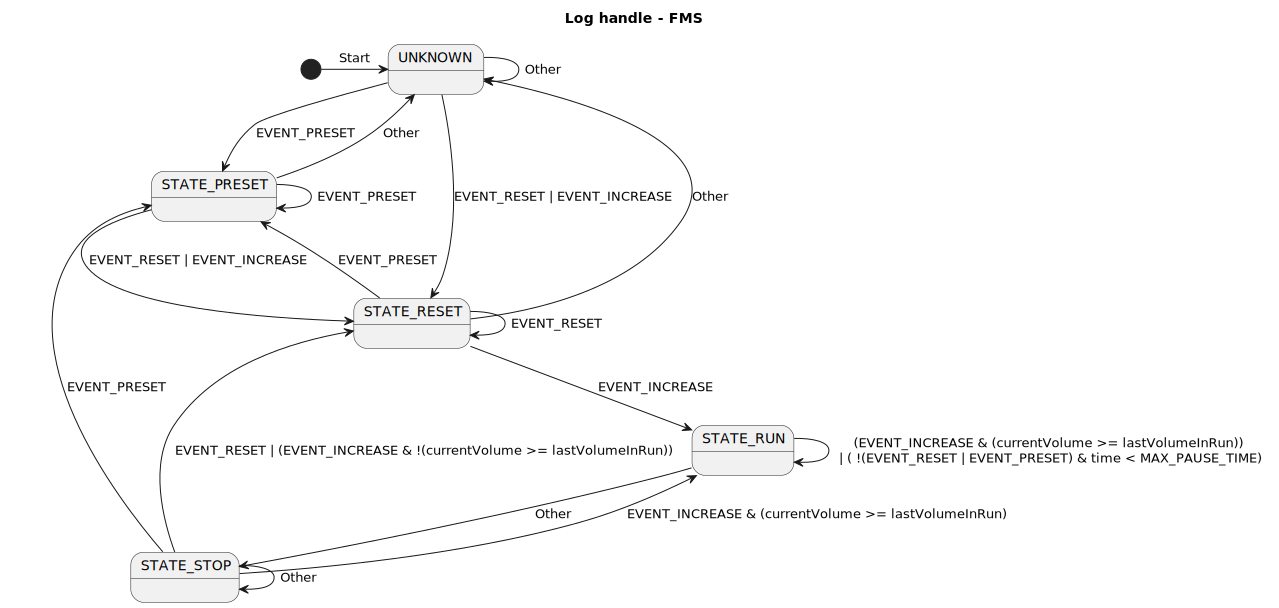
\includegraphics[width=1.0\linewidth]{Figures/LogProcess_Detect-machine-state.png}
    \caption{Sơ đồ trạng thái cho cột bơm}
    \label{fig:LogProcess_Detect-machine-state}
\end{figure}

Sau khi xác định trạng thái mới, hàm callback tương ứng được gọi để kiểm tra phiên bơm mới nếu có:


\begin{longtable}{|c|c|p{3cm}|p{6cm}|}
\hline
\textbf{Trạng thái cũ} & \textbf{Trạng thái mới} & \textbf{Hàm callback} & \textbf{Mô tả} \\
\hline
\endfirsthead

\hline
\textbf{Trạng thái cũ} & \textbf{Trạng thái mới} & \textbf{Hàm callback} & \textbf{Mô tả} \\
\hline
\endhead

\texttt{STATE\_PRESET} & \texttt{STATE\_PRESET} & Check overtime to cut preset & Kiểm tra xem màn hình ở trạng thái PRESET đã được giữ hơn 5 giây chưa. Nếu có, tạo một log mới cho preset. \\
\hline

\texttt{STATE\_RESET} & \texttt{STATE\_RUN} & Generate new Log & Tạo mới một log trống để bắt đầu ghi nhận dữ liệu màn hình. \\
\hline

\texttt{STATE\_RUN} & \texttt{STATE\_RUN} & Update Log info & Trong khi vẫn ở trạng thái RUN, hệ thống cập nhật thông tin log (ví dụ: thời gian, tiền, lít , đơn giá...). \\
\hline

\texttt{STATE\_RUN} & \texttt{STATE\_STOP} & Cut Log & Khi chuyển từ RUN sang STOP, hệ thống chốt log hiện tại  \\
\hline

\caption{Callback được gọi sau khi xác định trạng thái mới}
\label{tab:callback-when-machine-state-changed}
\end{longtable}

\FloatBarrier

\begin{figure}[!ht]
     \centering
    \includegraphics[width=1.0\linewidth]{Figures/flowcharts-DeviceService-OTA.png}
    \caption{Thuật toán thực hiện OTA trên Device Service}
    \label{fig:flowcharts-DeviceService-OTA}
\end{figure}


Các firmware file được gửi tới Device Service dạng base64-string, được kiểm tra tính hợp lệ sau đó lưu vào bộ nhớ tạm.

Khi có yêu cầu kích hoạt firmware, Device Service tiến hành:

\begin{itemize}
    \item Hỏi Thiết bị đọc màn hình file firmware cần cập nhật
    \item Chia file firmware được chọn dưới dạng các chunk độ dài 1000-byte 
    \item Gửi từng chunk tới Thiết bị đọc ghi màn hình cùng offset.
\end{itemize}


\FloatBarrier
\textbf{Thuật toán thực hiện OTA}

\textbf{API cho Client để giao tiếp với Device Service }

Device Service cung cấp API mở để bên Client UI hoặc các bên Client khác có thể giao tiếp để:

\begin{itemize}
    \item Nhận dữ liệu thời gian thực và các phiên bơm (log), trạng thái relay
    \item Yêu cầu cập nhật relay hoặc thực hiện OTA.
\end{itemize}

Dạng dữ liệu: JSON.

Giao thức: TCP.

Mỗi request message là 1 JSON bao gồm các trường

\begin{itemize}
    \item Message ID: UUID định danh message 
    \item Message Type: Loại message để phân loại nội dung.
    \item Và các trường khác là payload tùy thuộc vào Message Type.
\end{itemize}

Các Message Type được hỗ trợ:

\begin{longtable}{|c|p{11cm}|}
\hline
\textbf{MSG Type} & \textbf{Mô tả} \\
\hline
\endfirsthead

\hline
\textbf{MSG Type} & \textbf{Mô tả} \\
\hline
\endhead

0 & Báo cáo sự kiện Log/SubLog từ Device Service tới UI Client. Bao gồm thông tin log hoặc sublog được chốt trong quá trình sử dụng thiết bị. \\
\hline

1 & Báo cáo sự kiện đặt Preset từ Device Service tới UI Client. Được gửi khi nội dung preset không đổi trong 5s hoặc khi chuyển từ preset về reset. \\
\hline

2 & Yêu cầu từ UI Client tới Device Service để thay đổi trạng thái bật/tắt Relay và điều kiện tự động tắt Relay. \\
\hline

3 & Device Service báo cáo trạng thái của các Relay về UI Client. Có thể là phản hồi cho yêu cầu Set Relay hoặc báo cáo chủ động khi có thay đổi. \\
\hline

5 & UI Client gửi yêu cầu tải xuống file firmware về Device Service. File dưới dạng base64, chứa nội dung cần cập nhật cho thiết bị. \\
\hline

6 & UI Client yêu cầu Device Service kích hoạt firmware mới đã được tải xuống. Sau khi thực hiện, thiết bị sẽ tự động reset. \\
\hline

7 & UI Client yêu cầu Device Service trả về danh sách trạng thái hiện tại của tất cả các thiết bị đang quản lý. \\
\hline

8 & Device Service chủ động báo cáo trạng thái của một thiết bị đọc ghi màn hình (kết nối, loại thiết bị, phiên bản firmware...) về cho UI Client. \\
\hline

\caption{Danh sách các message\_type của Device Service}
\label{tab:message-types}
\end{longtable}

\FloatBarrier


Tạo các file log để quan sát tiến trình chạy (hình \ref{fig:logs-txt-files-when-start-DeviceService}):

\begin{itemize}
    \item \texttt{deviceInterface.txt}: file log cho khối Device Interface, ghi các thiết bị đã kết nối, kèm thông báo và lỗi trong quá trình chạy.
    \item \texttt{server-debug.txt}: file log thông báo và lỗi trong quá trình kết nối và giao tiếp Client UI.
    \item \texttt{UDPReport.txt}: Thông báo hiện trạng của tiến trình broadcast UDP.
\end{itemize}

\begin{figure}[!ht]
     \centering
    \includegraphics[width=1.0\linewidth]{Figures/logs-txt-files-when-start-DeviceService.png}
    \caption{Device Service: Các file logs}
    \label{fig:logs-txt-files-when-start-DeviceService}
\end{figure}
\FloatBarrier



% ======================== UI CLIENT ============





\subsubsection{Viết phần mềm Client UI hiển thị các phiên bơm}



\begin{itemize}
    \item Môi trường sử dụng: NodeJS v20.18.1
    \item Ngôn ngữ: TypeScript 
    \item Database: SQLite 
    \item Các thư viện chính sử dụng: ReactJS, sqlite3, MUI Components
\end{itemize}

Các bước triển khai:

Bước 1: Tạo cấu trúc dự án Electron

\begin{itemize}
    \item Sử dụng câu lệnh \texttt{npm create electron-vite@latest} để setup dự án.
    \item Chọn template là ReactJS, ngôn ngữ TypeScript, nhấn \texttt{enter} để bắt đầu tạo mẫu.
\end{itemize}



\begin{figure}[!ht]
     \centering
    \includegraphics[width=1.0\linewidth]{Figures/ElectronViteReact-template.png}
    \caption{Mẫu dự án sử dụng Electron + Vite + ReactJS}
    \label{fig:ElectronViteReact-template}
\end{figure}

\FloatBarrier

Bước 2: Triển khai các tác vụ ở Main Process bao gồm:

\begin{itemize}
    \item Tạo 2 TCP Client:
    \begin{itemize}
        \item Realtime Screen Device Service Client: để nghe dữ liệu màn hình thời gian thực, chuyển tiếp màn hình tới Render Process ở cổng 5001
        \item Event Device Service Client: để nhận phiên bơm (log), điều khiển relay ở cổng 5002. Các phiên bơm nhận được sẽ được chuyển tiếp tới Database ORM.
    \end{itemize}
    \item Tạo Database ORM để đọc ghi cơ sở dữ liệu phiên bơm.
\end{itemize}

Cơ sở dữ liệu phiên bơm gồm 1 bảng lưu các log/sublog gồm các trường:

\begin{figure}[!ht]
     \centering
    \includegraphics[width=0.4\linewidth]{Figures/DeviceService_log-info-entity.png}
    \caption{Các trường lưu trong bảng Log của Database}
    \label{fig:Database_log-info-entity}
\end{figure}

\FloatBarrier

Bước 3: Triển khai giao diện tại Renderer Process

Sử dụng MUI để xây dựng các component:

\begin{itemize}
    \item Khung hiển thị màn hình thiết bị (3 dòng).

    \item Bảng thống kê log/sublog theo thời gian thực.

    \item Lọc, tìm kiếm theo \texttt{device\_id}, \texttt{log\_id}, thời gian, trạng thái, ...

    \item Hiển thị trạng thái kết nối và relay theo từng thiết bị. Các nút điều khiển relay
\end{itemize}

\textbf{Giao diện hoàn chỉnh}
\begin{figure}[!ht]
     \centering
    \includegraphics[width=1\linewidth]{Figures/DeviceServiceClient-init-ui.png}
    \caption{Giao diện hiển thị Client UI}
    \label{fig:DeviceServiceClient-init-ui}
\end{figure}

 

\newpage


% CONCLUSIONS
\section*{KẾT LUẬN}
    \phantomsection\addcontentsline{toc}{section}{\numberline {}KẾT LUẬN}



\newpage

% REFERENCES
\phantomsection\addcontentsline{toc}{section}{\numberline {}TÀI LIỆU THAM KHẢO}

\bibliography{citation}
\newpage

% APPENDIX
\section*{PHỤ LỤC}
    \phantomsection\addcontentsline{toc}{section}{\numberline{} PHỤ LỤC}

    \setcounter{section}{0}
    \setcounter{subsection}{0}
        \setcounter{figure}{0}
            \setcounter{table}{0}

\appendix

\counterwithin{figure}{section}

% \section{Công trình công bố liên quan}\label{sec:cong_bo}

\section{Một số phương pháp đo và hiệu chuẩn}


Phụ lục cần thêm (nếu có)
...



\end{document}